\documentclass[11pt,a4paper]{article}
\usepackage[utf8]{inputenc}
\usepackage[german]{babel}
\usepackage{amsmath}
\usepackage{amsfonts}
\usepackage{amssymb}
\usepackage{float}
\usepackage{graphicx}
\usepackage{mwe}
\usepackage{changepage}
\usepackage[margin=100pt]{geometry}
\usepackage{tabularx}
\usepackage{color, colortbl}
\usepackage{multirow}
\usepackage{lmodern, textcomp}
\usepackage{fancyhdr}
\usepackage{lscape}
\usepackage{verbatim}
\usepackage{tikz}
\author{Georg Felber, Markus Mondl, Florian Ritter, Luca Wenzl}

\newenvironment{indentE}{\begin{adjustwidth}{0.5cm}{}}{\end{adjustwidth}}

\usepackage{xparse}

\ExplSyntaxOn
\NewDocumentCommand{\NewWeirdCommand}{mm}
{% #1 = command to define, #2 = replacement text
	\cs_new:Npn #1 ##1
	{
		\tl_set:Nn \l__simon_args_tl { ##1 }
		#2
	}
}
\NewDocumentCommand{\Arg}{m}
{
	\tl_item:Nn \l__simon_args_tl { #1 }
}

\tl_new:N \l__simon_parse_args_tl
\ExplSyntaxOff

\NewWeirdCommand{\UseCase}{\\\\
	\begin{table}[H]
		\begin{center}
			\begin{tabularx}{\linewidth}{|l|X|}
				\hline
				\multicolumn{2}{|c|}{\multirow{2}{*}{\large\textbf{\Arg{2}}}}\\
				\multicolumn{2}{|c|}{} \\
				\hline
				\multicolumn{2}{|l|}{\multirow{2}{*}{\large\textbf{UseCase}}}\\
				\multicolumn{2}{|l|}{} \\
				\hline\textbf{Art}&
				\Arg{1}\\
				%\rowcolor{LBlue}
				\hline\textbf{Beschreibung}&
				\Arg{4}\\
				\hline\textbf{Auslöser}&
				\Arg{5}\\
				%\rowcolor{LBlue} 
				\hline\textbf{Ergebnis}&
				\Arg{6}\\
				\hline\textbf{Akteure}&
				\Arg{7}\\
				%\rowcolor{LBlue}
				\hline\textbf{Informationen}&
				\Arg{8}\\
				\hline\textbf{Vorbedingungen}&
				\Arg{9}\\
				%\rowcolor{LBlue}
				\hline\textbf{Nachbedingung}&
				\Arg{10}\\
				\hline\textbf{Nutzen}&
				\Arg{11}\\
				%\rowcolor{LBlue}
				\hline\textbf{Aufwand}&
				\Arg{12}\\
				\hline\textbf{Priorität}& 
				\Arg{13}\\
				\hline
			\end{tabularx}
		\end{center}
	\end{table}
	\newpage
}

\pagestyle{fancy}
\lhead{Machbarkeitsstudie Phobos-Wireless}
\rhead{Team Phobos}
\lfoot{\hline \mbox{}\\ V1}
\cfoot{}
\rfoot{\hline \mbox{} \\ \thepage}

\title{Machbarkeitsstudie Phobos-Wireless}
\begin{document}
	\maketitle
	\thispagestyle{empty}
	\tikz[remember picture,overlay]
	\node[anchor=north east,inner sep=10pt] at (current page.north east)
	{
\includegraphics[height=3cm]{pictures/logo/logo.jpg}};
	\mbox{}\\
	\begin{table}[H]
		\begin{center}
			\begin{tabularx} {\linewidth}{|l|c|c|l|c|X|}
				\hline
				\textbf{V} & 
				\textbf{Autor} &
				\textbf{QS} & 
				\textbf{Datum} & 
				\textbf{Status} & 
				\textbf{Kommentar} \\
				\hline
				\multirow{2}{*}{0.1} & mmondl & \multirow{2}{*}{fritter} & \multirow{2}{*}{6.3.2019} & \multirow{2}{*}{Entwurf} & Analyse angefangen\\
				& gfelber & & & & Produktfunktionen
				angefangen\\
				\hline
				0.2 & gfelber & fritter & 13.3.2019 & Überarbeitet & Produktfunktionen\\
				\hline
				0.3 & mmondl & fritter & 14.3.2019 & Überarbeitet & Analyse verbessert, Zustände angefangen\\
				\hline
				0.4 & mmondl & fritter & 17.3.2019 & Überarbeitet & Zustände bearbeitet\\
				\hline
				0.5 & mmondl & fritter & 22.3.2019 & Überarbeitet & Risikoanalyse verbessert, Management Summary\\
				\hline
				0.6 & fritter & gfelber & 25.03.2019 & Überarbeitet & Technische Machbarkeit, Glossar\\
				\hline
				0.7 & fritter & gfelber & 25.03.2019 & Überarbeitet & Nutzwertanalyse\\
				\hline
				1.0 & gfelber & ZAKS & 26.03.2019 &  & Endversion\\
				\hline
			\end{tabularx}
		\end{center}
	\end{table}
	\end
	\newpage
	\tableofcontents
	\newpage
	\section{Einleitung}
Im Rahmen des Projekts wird das Projektteam eine Desktop-Applikation welche auf der Projektwebseite erhältlich ist, eine Mobile Version die für 5€ auf Google Play Store verfügbar ist, als auch die zuvor erwähnte Projektwebseite mit der das fertige Produkt vorgestellt wird, entwickelt. Die Webseite wird auch einen Shop enthalten mit welchem der Benutzer die Desktop-Applikation kaufen und downloaden kann. Die Benutzung der Webseite oder genauer gesagt dem Shop ist für jeden Besucher offen und benötigt daher keine Erstellung eines Benutzers.
\\\\
Genau wie bei der Verwendung der Webseite ist auch bei der Desktop-Applikation bzw. der Mobilen Version kein Benutzerprofil nötig. Bei beiden Applikationen muss der Benutzer zuerst den Empfänger auswählen und eine Verbindung mit diesem aufbauen. Nach dem erfolgreichen Verbindungsaufbau kann man mit nur einem Knopfdruck die zu versendende Datei auswählen und absenden. 			% Markus
	\section{Ist-Zustand}
Zu dem jetzigen Zeitpunkt ist die Nachfrage nach Datenübertragungs-Möglichkeiten definitiv da. Die Auswahl an Software, welche Cross Plattform Übertragung unterstützt, ist derzeit jedoch noch relativ gering. Es gibt zwar schon einige Möglichkeiten Daten zu übertragen, die meisten sind jedoch nur für ein bestimmtes Betriebssystem gedacht. Ebenfalls brauchen nur die wenigsten Applikationen keine stetige Internetverbindung.
\subsection*{Konkurrenzanalyse}
Weil es zu dem jetzigen Zeitpunkt noch keine Applikation gibt, welche die angeforderten Funktionen besitzt, ist dieses Projekt einzigartig. Es gibt zwar schon einige ähnliche Applikationen wie AirDrop für Apple Geräte und Zapya für Windows, diese erfüllen jedoch nicht die  Kernfunktionen welche das Produkt so einzigartig macht.\\\\
Hierbei erkennt AirDrop nur gewisse Apple Geräte welche in der nahen Umgebung des Benutzers sind  und hat dadurch keine Cross-Plattform Datenübertragung. Zu den verfügbaren Produkten gehört das iPhone, iPad, iPod Touch als auch jedes Mac Book und iMac mit dem Betriebssystem OS X 10.10 (Yosemite) oder neuer. Um eine erfolgreiche Datenübertragung mit AirDrop zu gewährleisten wird eine stetige Bluetooth Verbindung zwischen den Geräten als auch eine Internetverbindung benötigt.\\\\
Bei Zapya hingegen ist die Cross-Plattform Übertragung zwischen Windows, Android, iOS und Mac OS X möglich. Ebenfalls wird eine stetige Bluetooth Verbindung zwischen den benutzen Geräten benötigt. Im Gegensatz zu AirDrop muss für die Verwendung von Zapya jeoch keine Internetverbindung vorhanden sein. 			% Markus
	\section{Trendanalyse}
Es kommt immer wieder zu Situationen in denen man Medien oder verschiedenste andere Dateien zwischen 2 Geräten übertragen möchte. Oftmals treten diese Situationen auf dem Weg in die Arbeit bzw. Schule, in der Bus- bzw. Zugfahrt oder im Ausland ein. Genau in diesen Momenten sind oftmals nicht alle Kriterien für eine erfolgreiche Datenübertragung erfüllt.
\\\\
 Einer der wichtigsten Punkte welche für die Übertragung benötigt wird ist eine stetige Internetverbindung. Diese wird für die große Mehrheit an Übertragungssoftware benötigt. Da dies jedoch im Ausland oder in einem Tunnel während der Zugfahrt nicht der Fall ist, kann man die Daten nicht erfolgreich, auf das Empfängergerät, übertragen. Deshalb sind wir der Annahme das Projekt Phobos gerechtfertigt ist.
\\\\
Es wird angenommen das sich diese Projekt in Zukunft vielleicht in dessen Funktion und Nachfrage, durch die immer stärker werdende Digitalisierung an Wert verlieren wird. Nichtsdestotrotz wird vermutet das die Nachfrage trotz allem in Zukunft bestehen wird.				% Markus
	\section{Soll-Zustand}
Nach Abschluss des Projekts soll eine funktionsfähige Desktop-Applikation, Mobile Version als auch eine Projektwebseite geben. Die Applikationen sollen den kabellosen Datentransfer ermöglichen. Die Datenübertragung selber soll jedoch ohne jede Internetverbindung möglich sein. Die Verwendung der Produkte soll auch Cross Plattform unterstützten was es ermöglicht Daten zwischen Windows, Android und Linux zu übertragen.
\\\\
Die fertigen Produkte sollen alle eine eigene Verschlüsselung verwenden welche mit einem individuellen Verschlüsselungskey realisiert wird. Hierbei kann jeder Benutzer ,bevor er seine ausgewählten Daten versendet, seinen eigenen Key eintragen. Dieser Schlüssel muss dann auch auf dem Empfänger-Gerät eingetragen werden um die Daten wieder zu entschlüsseln.
\\\\
Die Applikationen sind nicht dazu gedacht die zu versendenden Dateien zu bearbeiten. Zur Bearbeitung zählt das verändern des Inhalts als auch die Veränderung des Dateinamens und Dateitypen. Ebenfalls soll in keiner der Produkte Werbung geben.
\\\\
Auf der Projektwebseite soll es einen Shop geben in dem sich jeder Besucher die Desktop-Applikation kaufen kann und herunterladen kann. Für die Verwendung der Funktionen der Webseite braucht der Besucher keinen Account. Ebenfalls soll die Mobile Version der Applikation auf Google Play Store hochgeladen werden wo es dann für 5€ erhältlich ist.			% Markus
 	\newpage
\section{Produktfunktionen}
Es werden die Funktionen anhand von verschieden Kriterien beschrieben. Diese können im genaueren aus der unteren Tabelle entnommen werden.
\UseCase{
	{Der Bereich, unter welchen die Funktionen fällt}
	{Der Name und die ID der Funktion}
	{Die Art, unter welche die Funktion in dessen Umsetzung fallen wird}
	{Eine kurze Beschreibung der Funktion.}
	{Der Grund für die Existenz der Funktion im Produkt.}
	{Das Ergebnis, welche die Funktion erfüllen soll.}
	{Die verschiedenen Teilnehmer, welche von dieser Funktion betroffen sind.}
	{Die ein- und ausgehenden Informationen welche in Zusammenhang mit dieser Funktion stehen.}
	{Die Bedingungen, welche von dem Eintreffen der Funktion herrschen.}
	{Die Bedingungen, welche nach dem Eintreffen der Funktion herrschen.}
	{Der Nutzen der Funktion: gering, mittel, hoch}
	{Der Aufwand der Funktion: gering, mittel, hoch}
	{Die Priorität der Funktion: Must Have, Should Have, Nice to Have}
}

\subsection{Desktop-Version}
Es werden die Funktionen beschrieben, welche die Desktop-Version des Produktes erfüllen soll. Diese werden grundsätzliche in Frontend und Backend unterteilt.
\subsubsection{Backend erstellen}
Das Backend umfasst alle Funktionen, welche vom Benutzer nicht gesehen werden können. Diese bearbeitet den Datentransfer, Datenaufbereitung und die Datensicherheit.
\paragraph{Aktivitätsdiagramm Backend}\mbox{}\\
\begin{figure}[H]
	\centering
	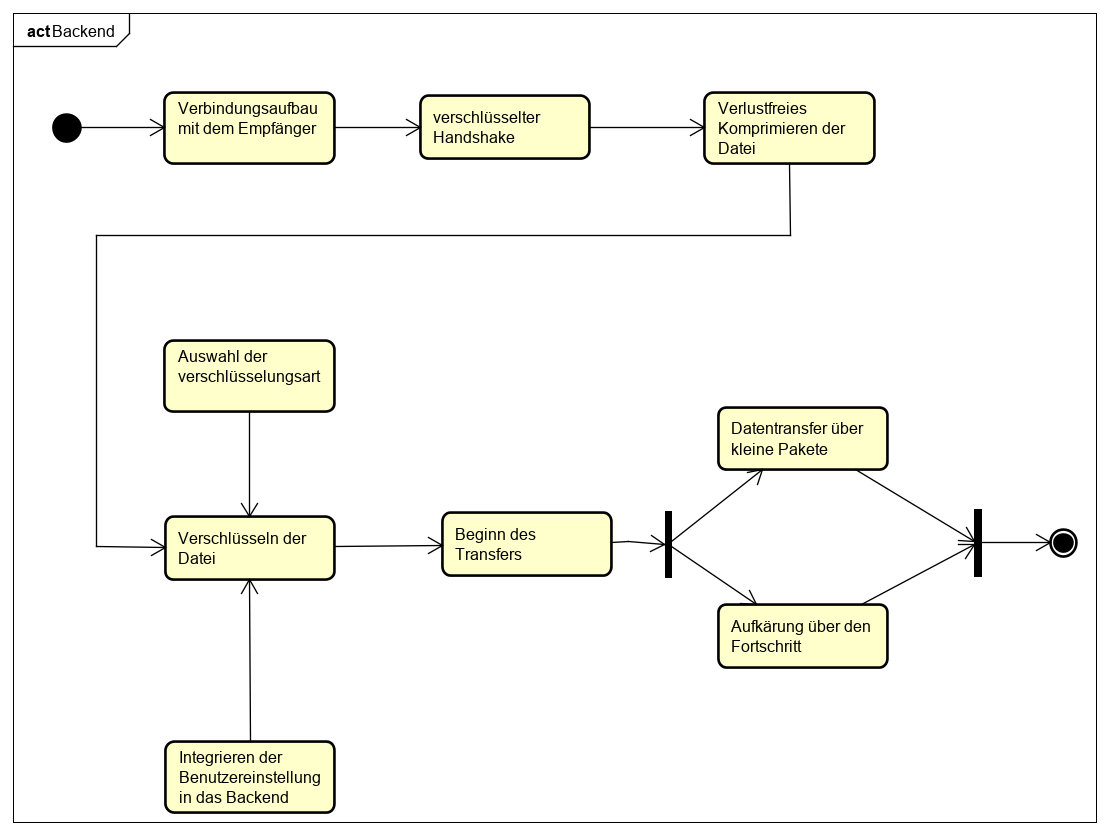
\includegraphics[width= 0.9\linewidth]{diagramms/activity/Backend.png}
	\caption{Aktivitätsdiagramm Backend}
\end{figure}
\newpage
\begin{indentE}\mbox{}
	\paragraph{/LF1110/ Verbindung aufbauen}\mbox{}\\
	Es wird die Verbindung mit dem ausgewählten Empfänger aufgebaut. Dieser Verbindungsaufbau besteht aus einem verschlüsselten Handshake, mit welchem die Systemdaten des Empfängers und Senders ausgetauscht werden. Wenn Empfänger und Sender den selben Verschlüsselungsschlüssel gewählt haben, ist der Handshake erfolgreich und der Transfer kann beginnen.
	\UseCase{
		{Desktop Backend}
		{/LF1110/ Verbindung aufbauen}
		{Backend}
		{Es wird die Verbindung mit dem Empfänger als Sender aufgebaut.}
		{Es muss eine Verbindung zwischen Empfänger und Sender für den Datentransfer herrschen}
		{Der Empfänger kann sich mit einem Empfänger der Wahl verbinden.}
		{Empfänger, Sender}
		{Sender, Namen }
		{Der Sender kann sich nicht mit dem Empfänger verbinden.}
		{Der Sender kann sich mit dem Empfänger verbinden.}
		{hoch}
		{mittel}
		{Must Have}
	}
	\paragraph{/LF1120/ Daten transferieren}\mbox{}\\
	Die Daten werden in kleinen Paketen versandt, um die Datensicherheit zu garantieren. Dabei haben diese eine einheitliche Größe und es werden unterschiedliche viele je nach Datengröße versandt. Dabei sollen der Empfänger und der Sender um den Fortschritt der Übertragung aufgeklärt werden.
	\UseCase{
		{Desktop Backend}
		{/LF1120/ Daten transferieren}
		{Backend}
		{Die Daten sollen vom Sender zum Empfänger transferiert werden. Diese soll dabei möglichst verlustlos gesendet werden.}
		{Der Daten müssen an den Empfänger gebracht werden.}
		{Die Daten des Sender kommen beim Empfänger an.}
		{Empfänger, Sender}
		{Datei(Name, Größe, Inhalt), Fortschritt(aus index und Anzahl Pakete), Sender, Empfänger}
		{Die Daten können dem Empfänger nicht vom Sender geschickt werden.}
		{Die Daten werden vom Sender zum Empfänger verlustlos gesendet.}
		{hoch}
		{gering}
		{Must Have}
	}
	\paragraph{/LF1130/ Daten komprimieren}\mbox{}\\
	Die Daten werden vor dem Versand verlustlos komprimiert, um die Datenmenge zu verkleinern. Die dabei gewählt Komprimierungsart, darf vom Auftragnehmer ausgewählt werden.
	\UseCase{
		{Desktop Backend}
		{/LF1130/ Daten komprimieren}
		{Backend}
		{Die Daten sollen vor dem Transfer verlustlos komprimiert werden, um die Übertragungsdauer zu verringern}
		{Der Datentransfer soll kürzer dauern.}
		{Der Datentransfer dauert in den meisten Fällen kürzer.}
		{Sender, Empfänger}
		{Daten}
		{Die Datenübertragung dauert länger.}
		{Die Datenübertragung dauert kürzer.}
		{mittel}
		{mittel}
		{Should Have}
	}
	\paragraph{/LF1140/ Datentransfer verschlüsseln}\mbox{}\\
	Der Datentransfer wird mit einem Verschlüsselungsschlüssel nach dem AES256 Standard verschlüsselt, um die Datensicherheit zu erhöhen. Diese wird dann vom Empfänger wieder entschlüsselt. Die dafür benutzte Verschlüsselungsart, kann vom Auftraggeber ausgewählt werden.
	\UseCase{
		{Desktop Backend}
		{/LF1140/ Datentransfer verschlüsseln}
		{Backend}
		{Der Datentransfer soll für eine höhere Sicherheit durch einen Schlüssel verschlüsselt werden.}
		{Der Datentransfer soll verschlüsselt stattfinden, damit die originalen Daten nicht von Dritten ausgelesen werden können.}
		{Der Datentransfer erfüllt den Standard AES256.}
		{Empfänger, Sender, Dritte}
		{Daten, Schlüssel}
		{Die originalen Daten können von Dritten ausgelesen werden}
		{Die originalen Daten sind während dem Transfer verschlüsselt}
		{mittel}
		{mittel}
		{Must Have}
	}
	\paragraph{/LF1150/ Benutzereinstellungen integrieren}\mbox{}\\
	Die vom Benutzer ausgewählten Benutzereinstellungen müssen in das Backend integrierte werden, um den Nutzen aus diesen Werten zu ziehen.
	\UseCase{
		{Desktop Backend}
		{/LF1150/ Benutzereinstellungen integrieren}
		{Backend}
		{Die Benutzereinstellungen sollen integriert werden.}
		{Die ausgewählten Benutzereinstellungen sollen in das Backend integriert werden.}
		{Die Einstellungen des Benutzer haben eine Auswirkung auf das Backend.}
		{Sender, Empfänger}
		{gewünschte Systemname, Verschlüsselung (Ja/Nein), Standardschlüssel, Speicherort}
		{Der Benutzer muss die meisten Daten bei jeder Übertragung neu einstellen, wodurch diese länger dauert}
		{Der Übertragung ist anpassbar, wodurch diese verschnellert werden kann. }
		{mittel}
		{gering}
		{Should Have}
	}
\end{indentE}
\subsubsection{Frontend erstellen}
Zu dem Frontend des Produktes gehören alle Elemente, auf welche der Benutzer Einsicht hat und mit denen er interagieren kann. Diese sind besonders für die Benutzbarkeit des Produkt wichtig, da diese die wichtigste Produktqualität ist.
\paragraph{Aktivitätsdiagramm Frontend}\mbox{}\\
\begin{figure}[H]
	\centering
	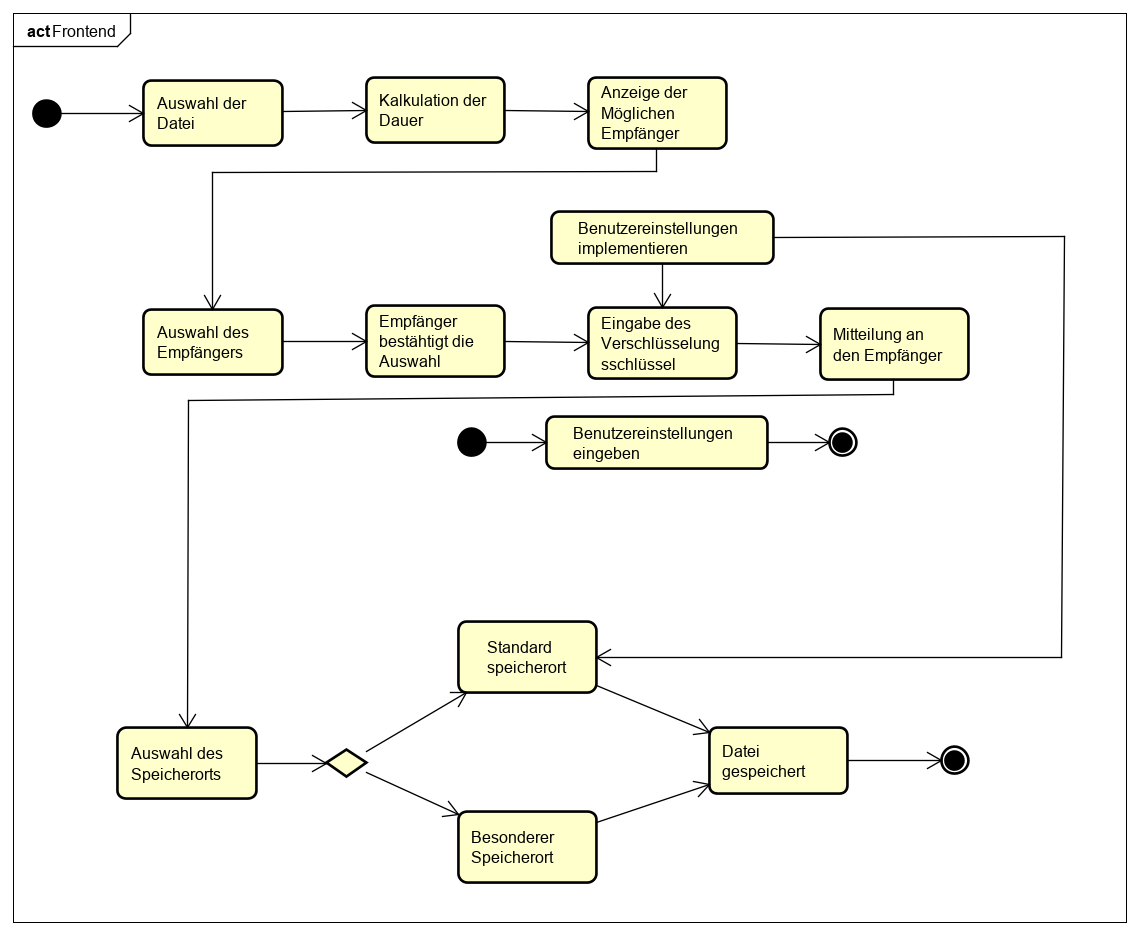
\includegraphics[width= 0.9\linewidth]{diagramms/activity/Frontend.png}
	\caption{Aktivitätsdiagramm Frontend}
\end{figure}
\newpage
\begin{indentE}\mbox{}
	\paragraph{/LF1210/ Datei auswählen}\mbox{}\\
	Der Benutzer wählt eine Datei aus, welche er verschicken möchte. Hierbei soll eine voreilige Kalkulation durchgeführt werden, welche die Dauer der Übertragung schätzt.
	\UseCase{
		{Desktop Frontend}
		{/LF1210/ Datei auswählen}
		{Frontend}
		{Ein wird die zu versendende Datei ausgewählt.}
		{Es muss die Datei, welche versendet werden soll, ausgewählt werden}
		{Es kann die Datei gesendet werden}
		{Sender}
		{Datei(Name, Größe, Inhalt)}
		{Es kann keine Datei ausgewählt werden}
		{Es kann eine zu versendende Datei ausgewählt werden}
		{hoch}
		{mittel}
		{Must Have}
	}
	\paragraph{/LF1220/ Empfänger auswählen}\mbox{}\\
	Es werden dem Benutzer die möglichen Empfänger angezeigt und ausgwählt oder er kann den Namen des Empfängers eingeben, um den Empfänger zu bestimmen. Dieser muss die Verbindung bestätigen.
	\UseCase{
		{Desktop Frontend}
		{/LF1220/ Empfänger auswählen}
		{Frontend}
		{Der Sender wählt anhand des Namens den Empfänger aus, mit dem der Datentransfer stattfinden soll.}
		{Es muss der Empfänger ausgewählt werden.}
		{Die Verbindung kann aufgebaut werden}
		{Sender, Empfänger}
		{Sendername, Empfängername}
		{Es kann kein Empfänger ausgewählt werden.}
		{Es kann anhand des Namens der Empfänger der Datei ausgewählt werden.}
		{hoch}
		{mittel}
		{Must Have}
	}
	\paragraph{/LF1230/ Verschlüsselungsschlüssel eingeben}\mbox{}\\
	Wenn kein Standard-Schlüssel ausgewählt ist, muss der Sender diesen bevor dem Verbindungsaufbau eingeben. Dieser muss dann dem Empfänger mitgeteilt werden und dieser muss den selben auch eingeben, um den Datentransfer zu ermöglichen.
	\UseCase{
		{Desktop Frontend}
		{/LF1230/ Verschlüsselungsschlüssel eingeben}
		{Frontend}
		{Es müssen Empfänger und Sender einen Schlüssel eingeben, die übereinstimmen, um den Datentransfer zu beginnen.}
		{Der Datentransfer muss mit einem Schlüssel verschlüsselt werden.}
		{Der Datentransfer kann verschlüsselt werden}
		{Sender, Empfänger}
		{Schlüssel}
		{Die Daten können nicht mit einem Schlüssel verschlüsselt werden}
		{Die Daten können mit einem frei wählbaren Schlüssel verschlüsselt werden}
		{hoch}
		{mittel}
		{Must Have}
	}
	\paragraph{/LF1240/ Datei speichern}\mbox{}\\
	Der Empfänger soll nach dem empfangen der Datei auswählen können, ob diese im Standard-Speicherort gespeichert wird, oder in einem besonderen. Wenn der Besondere ausgewählt worden ist, soll ihm ein Benutzerinterface gezeigt werden, indem er den Speicherort auswählen.
	\UseCase{
		{Desktop Frontend}
		{/LF1240/ Datei speichern}
		{Frontend}
		{Der Empfänger soll den Speicherort des bekommenen Datei auswählen können.}
		{Die Datei muss irgendwo gespeichert werden}
		{Der Speicherort der Datei kann ausgewählt werden}
		{Empfänger}
		{Datei(Name, Größe, Inhalt), Speicherort}
		{Die Datei wird entweder immer am selben Ort, oder nicht gespeichert}
		{Der Speicherort kann frei gewählt werden}
		{mittel}
		{gering}
		{Must Have}
	}
	\paragraph{/LF1250/ Benutzereinstellungen hinzufügen}\mbox{}\\
	Der Benutzer kann einige Fix-Einstellungen auf seinem Produkt tätigen. Darunter zählt die Möglichkeit, den Namen zu ändern, welcher den restlichen Nutzern angezeigt wird, die Verschlüsselung zu aktivieren oder deaktivieren, einen Standardschlüssel auszuwählen und einen Standard-Speicherort auszuwählen. Dabei sollen die eingegebenen Daten auf ihre Korrektheit überprüft werden.
	\UseCase{
		{Desktop Frontend}
		{/LF1250/ Benutzereinstellungen hinzufügen}
		{Frontend}
		{Der Benutzer kann verschiedenen Einstellungen tätigen, mit welche er die Datenübertragung beeinflussen kann.}
		{Die Einstellungen müssen auf einem Interface getätigt werden}
		{Die Einstellungen können getätigt werden}
		{Empfänger, Sender}
		{gewünschter Systemname, Verschlüsselung(Ja/Nein), Standardschlüssel, Standard-Speicherort}
		{Das Produkt kann nicht angepasst werden.}
		{Es können Einstellungen getroffen werden, welche das Produkt beeinflussen.}
		{mittel}
		{mittel}
		{Should Have}
	}
	\paragraph{/LF1260/ Desktopinterface designen}\mbox{}\\
	Es muss ein Interface für den Desktop entworfen werden. Dazu gehören Mockups und Prototypen. Diese müssen vor deren Implementierung vom Auftraggeber bestätigt werden.
	\UseCase{
		{Desktop Frontend}
		{/LF1260/ Desktopinterface designen}
		{Frontend}
		{Es müssen Mockups für die Desktopinterfaces erstellt werden. Diese diene als Vorlage für die Interfaces.}
		{Für einen schnellere und besser Implementierung sollen Mockups als Vorlage dienen.}
		{Die Implementierung ist einfacher, schneller und besser.}
		{Auftraggeber, Auftragnehmer}
		{}
		{Das Interface wird ohne Vorlage erstellt.}
		{Das Interface kann nach einer vom Auftraggeber bestätigten Vorlage erstellt werden.}
		{mittel}
		{gering}
		{Should Have}
	}
	\paragraph{/LF1270/ Desktopinterace implementieren}\mbox{}\\
	Das Desktopinterface muss nach der Bestätigung des Auftraggeber implementiert werden. 
	\UseCase{
		{Desktop Frontend}
		{/LF1270/}
		{Frontend}
		{Das Desktopinterface muss durch die Mockups realisiert werden.}
		{Der Benutzer hat keine Möglichkeit mit dem System zu integrieren}
		{Der Benutzer kann mit dem System interagieren und dadurch dessen Funktionen benutzen.}
		{Benutzer}
		{sämtliche Nutzereingaben}
		{Der Benutzer kann mit dem System nicht interagieren}
		{Der Benutzer ist in der Lage mit dem System zu interagieren}
		{hoch}
		{hoch}
		{Must-Have}
	}
	\paragraph{/LF1280/ Frontend und Backend verbinden}\mbox{}\\
	Es muss eine Verbindung zwischen dem Frontend und Backend erstellt werden, welche die Aufforderungen verarbeitet und zum Backend weiterleitet. Diese Verbindung, soll dem Benutzer entweder mitteilen, wie lange die Verarbeitung noch dauert oder bei kürzeren das wiederholte Aufrufen von Aufforderungen verhindern.
	\UseCase{
		{Desktop Frontend}
		{/LF1280/ Frontend und Backend verbinden}
		{Frontend}
		{Das Frontend muss mit dem Backend verbunden werden, um die Nutzereingaben an das Backend weiterzuleiten. Außerdem soll es Daten ans Frontend schicken, welche über momentane Prozess aufklärt.}
		{Die Daten müssen vom Frontend ans Backend und umgekehrt geschickt werden}
		{Das Frontend kann mit dem Backend und umgekehrt kommunizieren.}
		{Benutzer}
		{sämtliche Nutzereingaben und verwertete Daten}
		{Die Nutzerdaten können nicht an das Backend und die verwerteten Daten nicht ans Frontend geschickt werden.}
		{Daten können zwischen Frontend und Backend ausgetauscht werden.}
		{hoch}
		{mittel}
		{Must-Have}
	}
\end{indentE}
\subsection{App-Version}
Es werden die Funktionen beschrieben, welche die App-Version des Produktes erfüllen soll. Diese werden grundsätzliche in Frontend und Backend unterteilt.
\subsubsection{Backend erstellen}
Das Backend umfasst alle Funktionen, welche vom Benutzer nicht gesehen werden können. Diese bearbeitet den Datentransfer, Datenaufbereitung und die Datensicherheit.
\paragraph{Aktivitätsdiagramm Backend}\mbox{}\\
\begin{figure}[H]
	\centering
	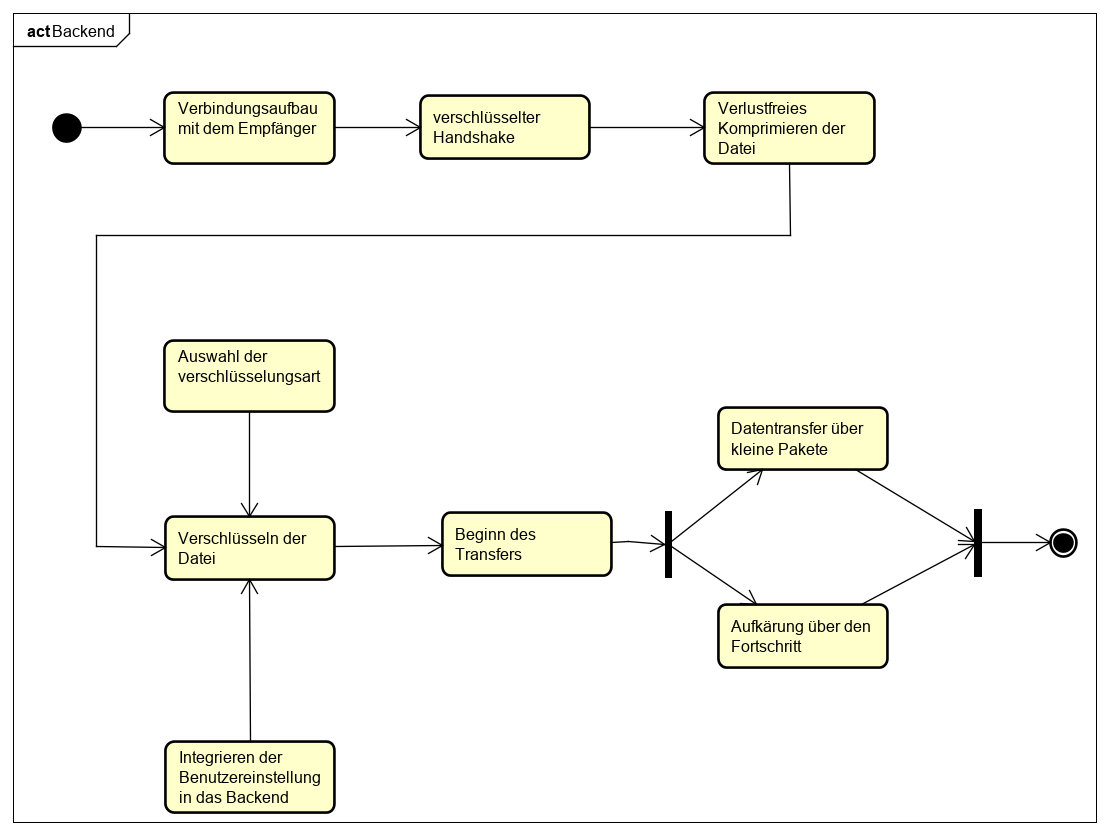
\includegraphics[width= 0.9\linewidth]{diagramms/activity/Backend.png}
	\caption{Aktivitätsdiagramm Backend}
\end{figure}
\newpage
\begin{indentE}\mbox{}
	\paragraph{/LF2110/ Verbindung aufbauen}\mbox{}\\
	Es wird die Verbindung mit dem ausgewählten Empfänger aufgebaut. Dieser Verbindungsaufbau besteht aus einem verschlüsselten Handshake, mit welchem die Systemdaten des Empfängers und Senders ausgetauscht werden. Wenn Empfänger und Sender den selben Verschlüsselungsschlüssel gewählt haben, ist der Handshake erfolgreich und der Transfer kann beginnen.
	\UseCase{
		{App Backend}
		{/LF2110/ Verbindung aufbauen}
		{Backend}
		{Es wird die Verbindung mit dem Empfänger als Sender aufgebaut.}
		{Es muss eine Verbindung zwischen Empfänger und Sender für den Datentransfer herrschen}
		{Der Empfänger kann sich mit einem Empfänger der Wahl verbinden.}
		{Empfänger, Sender}
		{Sender, Namen }
		{Der Sender kann sich nicht mit dem Empfänger verbinden.}
		{Der Sender kann sich mit dem Empfänger verbinden.}
		{hoch}
		{mittel}
		{Should Have}
	}
	\paragraph{/LF2120/ Daten transferieren}\mbox{}\\
	Die Daten werden in kleinen Paketen versandt, um die Datensicherheit zu garantieren. Dabei haben diese eine einheitliche Größe und es werden unterschiedliche viele je nach Datengröße versandt. Dabei sollen der Empfänger und der Sender um den Fortschritt der Übertragung aufgeklärt werden.
	\UseCase{
		{App Backend}
		{/LF2120/ Daten transferieren}
		{Backend}
		{Die Daten sollen vom Sender zum Empfänger transferiert werden. Diese soll dabei möglichst verlustlos gesendet werden.}
		{Der Daten müssen an den Empfänger gebracht werden.}
		{Die Daten des Sender kommen beim Empfänger an.}
		{Empfänger, Sender}
		{Datei(Name, Größe, Inhalt), Fortschritt(aus index und Anzahl Pakete), Sender, Empfänger}
		{Die Daten können dem Empfänger nicht vom Sender geschickt werden.}
		{Die Daten werden vom Sender zum Empfänger verlustlos gesendet.}
		{hoch}
		{gering}
		{Should Have}
	}
	\paragraph{/LF2130/ Daten komprimieren}\mbox{}\\
	Die Daten werden vor dem Versand verlustlos komprimiert, um die Datenmenge zu verkleinern. Die dabei gewählt Komprimierungsart, darf vom Auftragnehmer ausgewählt werden.
	\UseCase{
		{App Backend}
		{/LF2130/ Daten komprimieren}
		{Backend}
		{Die Daten sollen vor dem Transfer verlustlos komprimiert werden, um die Übertragungsdauer zu verringern}
		{Der Datentransfer soll kürzer dauern.}
		{Der Datentransfer dauert in den meisten Fällen kürzer.}
		{Sender, Empfänger}
		{Daten}
		{Die Datenübertragung dauert länger.}
		{Die Datenübertragung dauert kürzer.}
		{mittel}
		{mittel}
		{Nice to Have}
	}
	\paragraph{/LF2140/ Datentransfer verschlüsseln}\mbox{}\\
	Der Datentransfer wird mit einem Verschlüsselungsschlüssel nach dem AES256 Standard verschlüsselt, um die Datensicherheit zu erhöhen. Diese wird dann vom Empfänger wieder entschlüsselt. Die dafür benutzte Verschlüsselungsart, kann vom Auftraggeber ausgewählt werden.
	\UseCase{
		{App Backend}
		{/LF2140/ Datentransfer verschlüsseln}
		{Backend}
		{Der Datentransfer soll für eine höhere Sicherheit durch einen Schlüssel verschlüsselt werden.}
		{Der Datentransfer soll verschlüsselt stattfinden, damit die originalen Daten nicht von Dritten ausgelesen werden können.}
		{Der Datentransfer erfüllt den Standard AES256.}
		{Empfänger, Sender, Dritte}
		{Daten, Schlüssel}
		{Die originalen Daten können von Dritten ausgelesen werden}
		{Die originalen Daten sind während dem Transfer verschlüsselt}
		{mittel}
		{mittel}
		{Should Have}
	}
	\paragraph{/LF2150/ Benutzereinstellungen integrieren}\mbox{}\\
	Die vom Benutzer ausgewählten Benutzereinstellungen müssen in das Backend integrierte werden, um den Nutzen aus diesen Werten zu ziehen.
	\UseCase{
		{App Backend}
		{/LF2150/ Benutzereinstellungen integrieren}
		{Backend}
		{Die Benutzereinstellungen sollen integriert werden.}
		{Die ausgewählten Benutzereinstellungen sollen in das Backend integriert werden.}
		{Die Einstellungen des Benutzer haben eine Auswirkung auf das Backend.}
		{Sender, Empfänger}
		{gewünschte Systemname, Verschlüsselung (Ja/Nein), Standardschlüssel, Speicherort}
		{Der Benutzer muss die meisten Daten bei jeder Übertragung neu einstellen, wodurch diese länger dauert}
		{Der Übertragung ist anpassbar, wodurch diese verschnellert werden kann. }
		{mittel}
		{gering}
		{Nice to Have}
	}
\end{indentE}
\subsubsection{Frontend erstellen}
Zu dem Frontend des Produktes gehören alle Elemente, auf welche der Benutzer Einsicht hat und mit denen er interagieren kann. Diese sind besonders für die Benutzbarkeit des Produkt wichtig, da diese die wichtigste Produktqualität ist.
\paragraph{Aktivitätsdiagramm Frontend}\mbox{}\\
\begin{figure}[H]
	\centering
	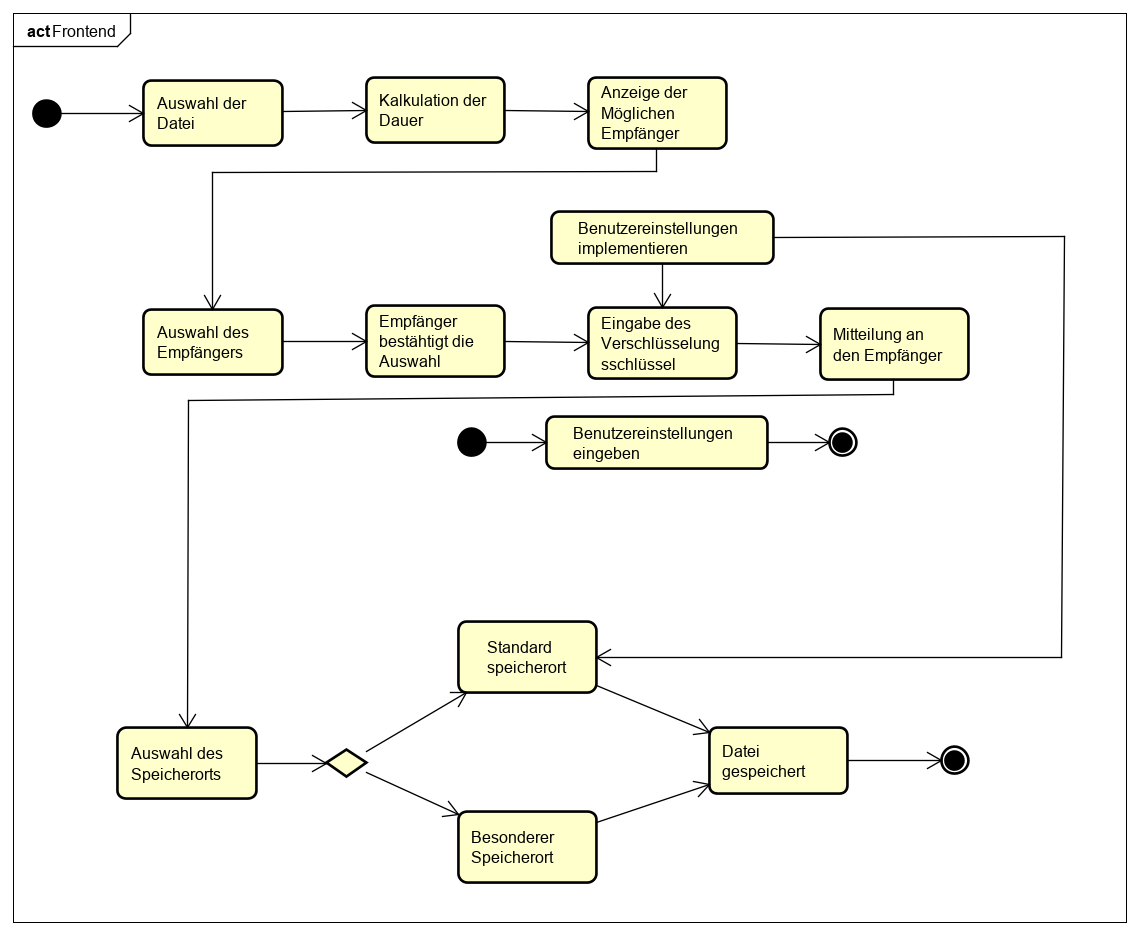
\includegraphics[width= 0.9\linewidth]{diagramms/activity/Frontend.png}
	\caption{Aktivitätsdiagramm Frontend}
\end{figure}
\newpage
\begin{indentE}\mbox{}
	\paragraph{/LF2210/ Datei auswählen}\mbox{}\\
	Der Benutzer wählt eine Datei aus, welche er verschicken möchte. Hierbei soll eine voreilige Kalkulation durchgeführt werden, welche die Dauer der Übertragung schätzt.
	\UseCase{
		{App Frontend}
		{/LF2210/ Datei auswählen}
		{Frontend}
		{Ein wird die zu versendende Datei ausgewählt.}
		{Es muss die Datei, welche versendet werden soll, ausgewählt werden}
		{Es kann die Datei gesendet werden}
		{Sender}
		{Datei(Name, Größe, Inhalt)}
		{Es kann keine Datei ausgewählt werden}
		{Es kann eine zu versendende Datei ausgewählt werden}
		{hoch}
		{mittel}
		{Should Have}
	}
	\paragraph{/LF2220/ Empfänger auswählen}\mbox{}\\
	Es werden dem Benutzer die möglichen Empfänger angezeigt und ausgwählt oder er kann den Namen des Empfängers eingeben, um den Empfänger zu bestimmen. Dieser muss die Verbindung bestätigen.
	\UseCase{
		{App Frontend}
		{/LF2220/ Empfänger auswählen}
		{Frontend}
		{Der Sender wählt anhand des Namens den Empfänger aus, mit dem der Datentransfer stattfinden soll.}
		{Es muss der Empfänger ausgewählt werden.}
		{Die Verbindung kann aufgebaut werden}
		{Sender, Empfänger}
		{Sendername, Empfängername}
		{Es kann kein Empfänger ausgewählt werden.}
		{Es kann anhand des Namens der Empfänger der Datei ausgewählt werden.}
		{hoch}
		{mittel}
		{Should Have}
	}
	\paragraph{/LF2230/ Verschlüsselungsschlüssel eingeben}\mbox{}\\
	Wenn kein Standard-Schlüssel ausgewählt ist, muss der Sender diesen bevor dem Verbindungsaufbau eingeben. Dieser muss dann dem Empfänger mitgeteilt werden und dieser muss den selben auch eingeben, um den Datentransfer zu ermöglichen.
	\UseCase{
		{App Frontend}
		{/LF2230/ Verschlüsselungsschlüssel eingeben}
		{Frontend}
		{Es müssen Empfänger und Sender einen Schlüssel eingeben, die übereinstimmen, um den Datentransfer zu beginnen.}
		{Der Datentransfer muss mit einem Schlüssel verschlüsselt werden.}
		{Der Datentransfer kann verschlüsselt werden}
		{Sender, Empfänger}
		{Schlüssel}
		{Die Daten können nicht mit einem Schlüssel verschlüsselt werden}
		{Die Daten können mit einem frei wählbaren Schlüssel verschlüsselt werden}
		{hoch}
		{mittel}
		{Should Have}
	}
	\paragraph{/LF2240/ Datei speichern}\mbox{}\\
	Der Empfänger soll nach dem empfangen der Datei auswählen können, ob diese im Standard-Speicherort gespeichert wird, oder in einem besonderen. Wenn der Besondere ausgewählt worden ist, soll ihm ein Benutzerinterface gezeigt werden, indem er den Speicherort auswählen.
	\UseCase{
		{App Frontend}
		{/LF2240/ Datei speichern}
		{Frontend}
		{Der Empfänger soll den Speicherort des bekommenen Datei auswählen können.}
		{Die Datei muss irgendwo gespeichert werden}
		{Der Speicherort der Datei kann ausgewählt werden}
		{Empfänger}
		{Datei(Name, Größe, Inhalt), Speicherort}
		{Die Datei wird entweder immer am selben Ort, oder nicht gespeichert}
		{Der Speicherort kann frei gewählt werden}
		{mittel}
		{gering}
		{Should Have}
	}
	\paragraph{/LF2250/ Benutzereinstellungen hinzufügen}\mbox{}\\
	Der Benutzer kann einige Fix-Einstellungen auf seinem Produkt tätigen. Darunter zählt die Möglichkeit, den Namen zu ändern, welcher den restlichen Nutzern angezeigt wird, die Verschlüsselung zu aktivieren oder deaktivieren, einen Standardschlüssel auszuwählen und einen Standard-Speicherort auszuwählen. Dabei sollen die eingegebenen Daten auf ihre Korrektheit überprüft werden.
	\UseCase{
		{App Frontend}
		{/LF2250/ Benutzereinstellungen hinzufügen}
		{Frontend}
		{Der Benutzer kann verschiedenen Einstellungen tätigen, mit welche er die Datenübertragung beeinflussen kann.}
		{Die Einstellungen müssen auf einem Interface getätigt werden}
		{Die Einstellungen können getätigt werden}
		{Empfänger, Sender}
		{gewünschter Systemname, Verschlüsselung(Ja/Nein), Standardschlüssel, Standard-Speicherort}
		{Das Produkt kann nicht angepasst werden.}
		{Es können Einstellungen getroffen werden, welche das Produkt beeinflussen.}
		{mittel}
		{mittel}
		{Nice to Have}
	}
	\paragraph{/LF2260/ Appinterface designen}\mbox{}\\
	Es muss ein Interface für das Smartphone entworfen werden. Dazu gehören Mockups und Prototypen. Diese müssen vor deren Implementierung vom Auftraggeber bestätigt werden.
	\UseCase{
		{App Frontend}
		{/LF2260/ Appinterface designen}
		{Frontend}
		{Es müssen Mockups für die Appinterfaces erstellt werden. Diese diene als Vorlage für die Interfaces.}
		{Für einen schnellere und besser Implementierung sollen Mockups als Vorlage dienen.}
		{Die Implementierung ist einfacher, schneller und besser.}
		{Auftraggeber, Auftragnehmer}
		{}
		{Das Interface wird ohne Vorlage erstellt.}
		{Das Interface kann nach einer vom Auftraggeber bestätigten Vorlage erstellt werden.}
		{mittel}
		{gering}
		{Nice to Have}
	}
	\paragraph{/LF2270/ Appinterface implementieren}\mbox{}\\
	Das Appinterface muss nach der Bestätigung des Auftraggeber implementiert werden. 
	\UseCase{
		{App Frontend}
		{/LF2270/ Appinterface implementieren}
		{Frontend}
		{Das Appinterface muss durch die Mockups realisiert werden.}
		{Der Benutzer hat keine Möglichkeit mit dem System zu integrieren}
		{Der Benutzer kann mit dem System interagieren und dadurch dessen Funktionen benutzen.}
		{Benutzer}
		{sämtliche Nutzereingaben}
		{Der Benutzer kann mit dem System nicht interagieren}
		{Der Benutzer ist in der Lage mit dem System zu interagieren}
		{hoch}
		{hoch}
		{Should Have}
	}
	\paragraph{/LF2280/ Frontend und Backend verbinden}\mbox{}\\
	Es muss eine Verbindung zwischen dem Frontend und Backend erstellt werden, welche die Aufforderungen verarbeitet und zum Backend weiterleitet. Diese Verbindung, soll dem Benutzer entweder mitteilen, wie lange die Verarbeitung noch dauert oder bei kürzeren das wiederholte Aufrufen von Aufforderungen verhindern.
	\UseCase{
		{App Frontend}
		{/LF2280/ Frontend und Backend verbinden}
		{Frontend}
		{Das Frontend muss mit dem Backend verbunden werden, um die Nutzereingaben an das Backend weiterzuleiten. Außerdem soll es Daten ans Frontend schicken, welche über momentane Prozess aufklärt.}
		{Die Daten müssen vom Frontend ans Backend und umgekehrt geschickt werden}
		{Das Frontend kann mit dem Backend und umgekehrt kommunizieren.}
		{Benutzer}
		{sämtliche Nutzereingaben und verwertete Daten}
		{Die Nutzerdaten können nicht an das Backend und die verwerteten Daten nicht ans Frontend geschickt werden.}
		{Daten können zwischen Frontend und Backend ausgetauscht werden.}
		{hoch}
		{mittel}
		{Should Have}
	}
\end{indentE}
\subsection{Publizierung}
Um mit dem Produkt etwas zu erwirtschaften, muss dieses der Zielgruppe anschaulich gemacht werden. Dabei ist die größe der Plattformen und die Anzahl der Plattformen, welche dies machen, für ein erfolgreiches Produkt besonders wichtig.
\paragraph{Aktivitätsdiagramm Publizierung}\mbox{}\\
\begin{figure}[H]
	\centering
	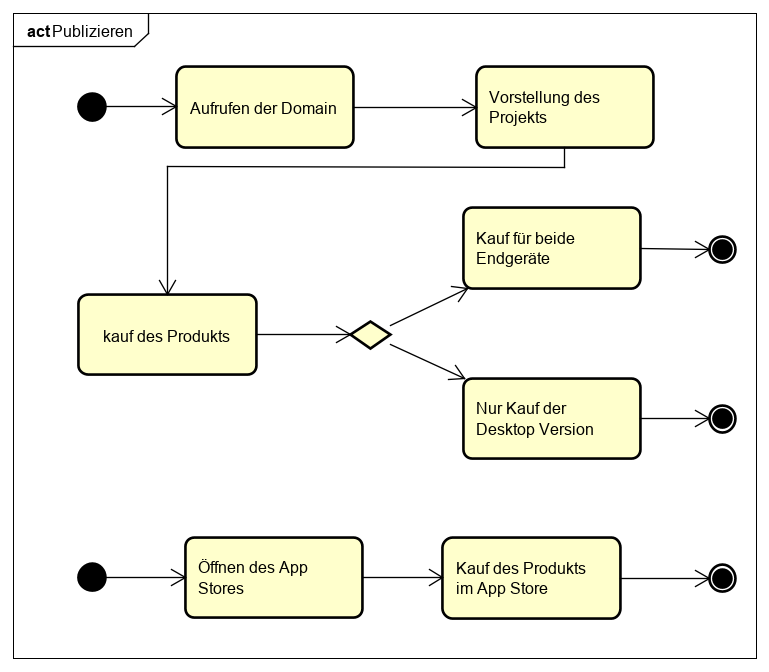
\includegraphics[width= 0.9\linewidth]{diagramms/activity/Publizieren.png}
	\caption{Aktivitätsdiagramm Publizierung}
\end{figure}
\newpage
\begin{indentE}\mbox{}
	\paragraph{/LF3110/ Website erstellen}\mbox{}\\
	Es wird eine Webseite erstellt, auf welche das Produkt vorgestellt wird. Außerdem soll diese dem Besucher das Projektteam und den Auftraggeber näher bringen, auf einer eigenen About-Seite. Diese Webseite wird dann auf einen Hosting-Provider hochgeladen, von wo sie mit einer Domain aufgerufen werden kann.
	\UseCase{
		{Publizierung}
		{/LF3110/ Website erstellen}
		{Publizierung}
		{Es wird eine Webseite erstellt, auf welche das Produkt publiziert werden soll. Diese soll außerdem auf das Projektteam aufmerksam machen und über das Internet mit einer Domain erreichbar sein.}
		{Das Produkt soll auf einer Webseite publiziert werden, und den potenziellen Kunden das Projektteam näher gebracht werden.}
		{Das Produkt ist im Internet auffindbar}
		{Benutzer, Projektteam (Auftraggeber + Auftragnehmer)}
		{Produktinformationen, Projektteam}
		{Das Produkt kann nicht über eine Webseite aufgefunden werden.}
		{Das Produkt ist über ein Webseite auffindbar}
		{hoch}
		{gering}
		{Must Have}
	}
	\paragraph{/LF3120/ Produkt auf Webseite veröffentlichen}\mbox{}\\
	Das Produkt muss auf ihrer eigenen Webseite /LF2060/ publiziert werden. Diese besitzt eine eigne Seite für den Download der Software. Dort kann man die App und Desktop Version für 5€ kaufen und die Desktop Version einzeln für 3€.
	\UseCase{
		{Publizierung}
		{LF3120/ Produkt auf Webseite veröffentlichen}
		{Publizierung}
		{Das Produkt soll von der Webseite gedownloadet werden können. Dabei soll die App und Desktop Version für 5 € gemeinsame und die Desktop Version einzeln für 3€ angeboten werden.}
		{Das Produkt muss für den potenziellen Kunden erwerbbar sein}
		{Das Produkt kann auf der Webseite automatisiert verkauft werden}
		{potenzieller Kunde}
		{Zahlungsinformationen, Produkt (als Download)}
		{Das Produkt ist für den potenziellen Kunden nicht erwerbbar}
		{Das Produkt kann auf der Webseite verwirtschaftet werden}
		{hoch}
		{mittel}
		{Must Have}
	}
	\paragraph{/LF3210/ Produkt auf Play Store veröffentlichen}\mbox{}\\
	Die Android App soll auf dem Google Play Store hochgeladen werden und dort für eine Preis von 3€ verkauft werden. Dafür muss ein Google Developer Account erstellt werden, um diese hochzuladen.
	\UseCase{
		{Publizierung}
		{/LF3210/ Produkt auf Play Store veröffentlichen}
		{Publizierung}
		{Die App-Version wird auf dem Play Store veröffentlicht, wo sie für 3€ erwerbt werden kann.}
		{Es soll die potenzielle Kundschaft erhöht werden, indem ie App-Version auch auf dem Play-Store verfügbar ist.}
		{Es wird eine größter Kundschaft(Android) angesprochen}
		{potenzielle Kunden}
		{App-Version(als Download)}
		{Der Erwerb wird nicht auf dem Play Store angeboten.}
		{Der Erwerb ist über den Play Store möglich}
		{mittel}
		{gering}
		{Should Have}
	}
	\paragraph{/LF3220/ Produkt auf App Store veröffentlichen}\mbox{}\\
	Die iOS App kann auf dem Apple App Store hochgeladen werden und dort für 3€ verkauft werden.
	\UseCase{
		{Publizierung}
		{/LF3220/ Produkt auf App Store veröffentlichen}
		{Publizierung}
		{Die App-Version wird auf dem App Store veröffentlicht, wo sie für 3€ erwerbt werden kann.}
		{Es soll die potenzielle Kundschaft erhöht werden, indem ie App-Version auch auf dem App Store verfügbar ist.}
		{Es wird eine größter Kundschaft(iOS) angesprochen}
		{potenzielle Kunden}
		{App-Version(als Download)}
		{Der Erwerb wird nicht auf dem App Store angeboten.}
		{Der Erwerb ist über den App Store möglich}
		{mittel}
		{mittel}
		{Nice to Have}
	}
\end{indentE}		% Georg
	\section{Machbarkeit}
Das Projekt wird anhand seine wirtschaftlichen und technischen Machbarkeit analysiert. Dabei sol sich herausstellen ob der Beginn des gerechtfertigt ist, und wie dessen Umsetzung ausschauen soll.
\subsection{Technische Machbarkeit}
Es wird die technische Machbarkeit des Projektes anhand seiner Umsetzungsmöglichkeiten analysiert und die am besten geeigneten Option gewählt.
\subsubsection{Programmiersprache}
Um eine einfache und umfangreiche Programmierung zu ermöglichen wird die betriebssystemunabhängige Programmiersprache Java zum Einsatz kommen. Die Funktionalitäten dieser Sprache umfassen die Anforderungen des Projekts und sind dem Projektteam im Allgemeinen bekannt.
\subsubsection{Verschlüsselung}
Verschlüsselungsarten haben Vor- und Nachteile. Diese werden in den folgenden Paragrafen behandelt und ausführlich beschrieben.
\begin{indentE}\mbox{}
	\paragraph{AES256}\mbox{}\\
	AES256 ist eine schlüsselbasierte Verschlüsselung mit einem 256 Bit Algorithmus. Dies bedeutet, dass ein zu verschlüsselndes Zeichen zu einer nach dem Schlüssel generierten Zeichenkette von 256 Zeichen wird. Dies erhöht die Sicherheit, wirkt sich jedoch auf den Speicher aus, da mehrere Zeichen mehr Speicherverbrauch bedeuten.
	
	\paragraph{Benutzerdefiniert}\mbox{}\\
	Eine benutzerdefinierte Verschlüsselung ist meist die sicherste Methode, da man hierzu keine öffentlichen Entschlüsselungsverfahren finden kann. Sie sind jedoch sehr aufwendig zu erstellen und erfordern viel Fachwissen.
	
	\paragraph{Kodierung}\mbox{}\\
	Kodierungen sind im Gegensatz zu Verschlüsselungen einheitlich. Sie haben die selben Muster und können mit Hilfe von Online-Methoden innerhalb von wenigen Sekunden dekodiert werden. Diese Art von Sicherheit ist sehr einfach zu implementieren und erfordert keinen großen Aufwand. Sie ist jedoch die Unsicherste von allen Methoden.
	
	\paragraph{Nutzwertanalyse}\mbox{}\\
	Die Analyse des Nutzwertes der Verschlüsselungsmethode zeigt, welche Art am besten geeignet ist. Da die Sicherheit der Methode im Vordergrund steht, ist es wichtig Wert darauf zu legen und dies als größten Entscheidungsfaktor zu definieren. Durch den Zusammenhang der Schnelligkeit, der Einfachheit und der Effizienz bildet sich mithilfe der Sicherheit eine einheitliche Nutzwertstatistik, die dazu führen lässt, dass die Verschlüsselung AES256 eher geeignet ist, als die Konkurrenz.
	\begin{table}[H]
		\begin{center}
			\begin{tabularx} {\linewidth}{|X|c|c|c|c|c|c|c|}
				\hline
				\multicolumn{2}{|c|}{\textbf{Kriterien}} & 
				\multicolumn{2}{c|}{\textbf{AES256}} &
				\multicolumn{2}{c|}{\textbf{Benutzerdef.}} & 
				\multicolumn{2}{c|}{\textbf{Kodierung}} \\
				\hline
				Sicherheit & 40\% & Anteil & 18\% & Anteil & 22\% & Anteil & 0\% \\
				\hline
				Schnelligkeit & 20\% & Anteil & 5\% & Anteil & 4\% & Anteil & 11\% \\
				\hline
				Einfachheit & 30\% & Anteil & 12\% & Anteil & 3\% & Anteil & 15\% \\
				\hline
				Effizienz & 10\% & Anteil & 5\% & Anteil & 4\% & Anteil & 1\% \\
				\hline
				Eignung & 100\% &  & 40\% &  & 33\% &  & 27\% \\
				\cline{1-2}\cline{4-4}\cline{6-6}\cline{8-8}
			\end{tabularx}
		\end{center}
	\end{table}
\end{indentE}

\subsubsection{Datentransfer}
Die meist genutzten Technologien des heutigen Datentransfers für Mobilgeräte werden in Einzelheiten beschrieben und konkret analysiert.
\begin{indentE}\mbox{}
	\paragraph{WLAN}\mbox{}\\
	Eine kabellose Internetverbindung wie WLAN ist in der Lage, eine schnelle Datenbrücke aufzubauen und mehrere Geräte gleichzeitig zu verbinden. Bei WLAN-Verbindungen finden jedoch häufig Unterbrechungen statt, da es beispielsweise nicht durch Stahlwände hindurchstrahlt, da es eine hohe Frequenz hat. Weiters ist es keine Herausforderung Daten über WLAN abzuhören, da es einen großen Radius hat und zudem standardisierte Verschlüsselungen nutzt.
	
	\paragraph{BlueTooth}\mbox{}\\
	BlueTooth ist eine kabellose Technologie, welche bei Kurzstreckendatenverbindungen eingesetzt wird und eine niedrige Frequenz nahe der Radiowellen benutzt. Es ist dementsprechend langsamer als WLAN. BlueTooth ist nicht in der Lage mehr als einen Empfänger zu haben kann jedoch Daten ohne einer Internetverbindung transferieren. Die Datenbrücke über einen RFCOMM-Channel ist sehr sicher, da sie im PAN-Betrieb keine große Reichweite hat, um abgehört zu werden.
	
	\paragraph{Nutzwertanalyse}\mbox{}\\
	Die Analyse des Nutzwertes der Verbindungstechnologie zeigt, welche Art am besten geeignet ist. Hierbei steht die Abhörsicherheit im Mittelpunkt der Faktoren. Gemeinsam mit der Reichweite, der Stärke und der Geringhäufigkeit bildet sie eine stark geneigte Eignung zur BlueTooth-Technologie. Das Ergebnis besagt nun, dass die Verwendung von BlueTooth mehr geeignet ist, als die ihrer Konkurrenz.
	\begin{table}[H]
		\begin{center}
			\begin{tabularx} {\linewidth}{|X|c|c|c|c|c|}
				\hline
				\multicolumn{2}{|c|}{\textbf{Kriterien}} & 
				\multicolumn{2}{c|}{\textbf{WLAN}} &
				\multicolumn{2}{c|}{\textbf{BlueTooth.}} \\
				\hline
				Reichweite & 10\% & Anteil & 8\% & Anteil & 2\% \\
				\hline
				Abhörsicherheit & 40\% & Anteil & 4\% & Anteil & 36\% \\
				\hline
				Stärke & 20\% & Anteil & 13\% & Anteil & 7\%  \\
				\hline
				Geringhäufigkeit & 30\% & Anteil & 3\% & Anteil & 27\%  \\
				\hline
				Eignung & 100\% &  & 28\% &  & 72\%\\
				\cline{1-2}
				\cline{4-4}
				\cline{6-6}
			\end{tabularx}
		\end{center}
	\end{table}
\end{indentE}
\subsubsection{Kompression}
Im Folgenden werden zwei Arten der Kompression beschrieben und es wird zu einer detaillierten Nutzwertanalyse gegriffen.
\begin{indentE}\mbox{}
	\paragraph{Verlustfreie Kompression}\mbox{}\\
	Eine verlustfreie Kompression komprimiert die gegebenen Daten so, dass mehrfache Inhalte kleiner zusammengefasst werden und beim dekomprimieren wieder ausgebreitet werden. Diese Methode ist nicht die effektivste, sie ist jedoch für wichtige Daten, die keine Verluste aufweisen dürfen sehr geeignet. Sie ist zudem schnell, geben jedoch nicht die meiste Menge an Speicherplatz frei. ZIP und RAR sind Beispiele für solch eine Kompressionsart. 
	
	\paragraph{Verlustbehaftete Kompression}\mbox{}\\
	Die effektivsten Methoden zur Komprimierung sind verlustbehaftete Kompressionen, da sie viele unnötige Details einfach entfernen. Nachteil ist auch, dass die Inhalte erst einmal gelöscht werden müssen und diese Methode dadurch etwas langsamer ist. Solch Methoden werden meist vereinzelt in eigenen Dateiformaten wie MP3 und JPEG eingesetzt.
	
	\paragraph{Nutzwertanalyse}\mbox{}\\
	Die Analyse des Nutzwertes der Kompressionsmethode zeigt, welche Art am besten geeignet ist. Eindeutiger Weise ist die Schnelligkeit, da BlueTooth die langsamere Übertragungsraten besitzt, im Mittelpunkt. Auch wenn die Kompressionsrate bei der Konkurrenz von ZIP wesentlich besser wäre, ist es effizienter diese Methode aus Gründen der Konsistenz und Schnelligkeit zu wählen.
	\begin{table}[H]
		\begin{center}
			\begin{tabularx} {\linewidth}{|X|c|c|c|c|c|c|c|}
				\hline
				\multicolumn{2}{|c|}{\textbf{Kriterien}} & 
				\multicolumn{2}{c|}{\textbf{ZIP}} &
				\multicolumn{2}{c|}{\textbf{RAR}} & 
				\multicolumn{2}{c|}{\textbf{Benutzerdef.}} \\
				\hline
				Schnelligkeit & 60\% & Anteil & 30\% & Anteil & 18\% & Anteil & 12\% \\
				\hline
				Kompressionsrate & 30\% & Anteil & 9\% & Anteil & 15\% & Anteil & 6\% \\
				\hline
				Konsistenz & 10\% & Anteil & 6\% & Anteil & 3\% & Anteil & 1\% \\
				\hline
				Eignung & 100\% &  & 45\% &  & 36\% &  & 19\% \\
				\cline{1-2}\cline{4-4}\cline{6-6}\cline{8-8}
			\end{tabularx}
		\end{center}
	\end{table}
\end{indentE}
\subsection{Wirtschaftliche Machbarkeit}
Es wird der Aufwand welcher für das Projektteam anfällt beschrieben. Ebenfalls werden die verschiedenen Risiken welche auftreten können erklärt und in einer Risikomatrix visuell dargestellt.
\subsubsection{Personalaufwand}
Allgemein kann man es in 3 größere Teile einteilen. Einmal der Entwicklung der Desktop-Version, auf welche hohe Priorität gelegt wird, einmal die Erstellung einer Mobiltelefon-Applikation und zuletzt die Entwicklung eines Webportals auf dem das Produkt vorgestellt wird. Diese 3 Teile kann man erneut in 2 Teile teilen nämlich Back-End und Front-End.
\\
All das wird einiges an Durchführungszeit beanspruchen weswegen alle Entwickler Zeitgleich an dem Projekt arbeiten. Insgesamt wird das Projekt 200 Stunden zur Fertigstellung brauchen, wobei jeder im Projektteam ungefähr gleichlang daran arbeitet.
\newpage
\subsubsection{Risikoanalyse}
Bei diesem Projekt sind, genau wie bei jedem anderen auch, Risiken nicht vermeidbar. Einer dieser Risiken könnte eventuelle Abwesenheit sein. Falls dieser Fall in Kraft treten sollte werden die restlichen Entwickler im Projektteam den fehlenden Teil übernehmen.
\begin{table}[H]
	\begin{center}
		\begin{tabularx} {\linewidth}{
				|c|X|c|c|c|c|X|
			}
			\hline
			\footnotesize \multirow{3}{\dimexpr.125\linewidth-2\tabcolsep-1.3333\arrayrulewidth}{Arbeits-paket}&\multirow{3}{*}{Projektrisiko}&\multirow{3}{\dimexpr.1\linewidth-2\tabcolsep-1.3333\arrayrulewidth}{\scriptsize Wahr-schein-lichkeit}&\multicolumn{3}{c|}{\multirow{2}{*}{Auswirkung auf}}&\multirow{3}{*}{Gegenstrategie}\\
			& & & \multicolumn{3}{c|}{} &\\
			\cline{4-6}
			&&&\scriptsize Qualität&\scriptsize Kosten&\scriptsize Zeit&\\
			\hline
			1.1 & Deadline nicht eingehalten & 5\% & 0 & 0 € & +10h & Proaktiv: Arbeitseinteilung besser planen Reaktiv: Bessere Zeitplanung\\
			\hline
			1.2 & Konflikt im Team & 15\% & 2 & 0 € & +8h & Proaktiv: Teambildung fördern \newline Reaktiv: Konflikt besprechen\\
			\hline
			1.3 & Arbeits-verweigerung & 5\% & 2 & 0 € & +10h & Proaktiv: Teambildung fördern Reaktiv: Konflikt besprechen \\
			\hline
			1.4 & Deadline nicht eingehalten & 5\% & 0 & 0 € & +10h & Proaktiv: Arbeitseinteilung besser planen \newline Reaktiv: Überstunden einarbeiten\\
			\hline
			2.1.1 & Aufwändige Aufsetzung & 15\% & 1 & 0 € & +3h & Proaktiv: Bekannte Software verwenden \newline Reaktiv: Experten fragen\\
			\hline
			2.1.2 & Verringerte Funktionalität & 5\% & 3 & 50 € & +10h & Proaktiv: Funktionen aufteilen \newline Reaktiv: Meeting mit Auftraggeber\\
			\hline
			2.1.3 & Sicherheitslücken & 10\% & 2 & 150 € & +10h & Proaktiv: Ausführliches Testen \newline Reaktiv: Patches herausbringen\\
			\hline
		\end{tabularx}
	\end{center}
\end{table}
\newpage
\begin{table}[H]
	\begin{center}
		\begin{tabularx} {\linewidth}{
				|c|X|c|c|c|c|X|
			}
			\hline
			\footnotesize \multirow{3}{\dimexpr.125\linewidth-2\tabcolsep-1.3333\arrayrulewidth}{Arbeits-paket}&\multirow{3}{*}{Projektrisiko}&\multirow{3}{\dimexpr.1\linewidth-2\tabcolsep-1.3333\arrayrulewidth}{\scriptsize Wahr-schein-lichkeit}&\multicolumn{3}{c|}{\multirow{2}{*}{Auswirkung auf}}&\multirow{3}{*}{Gegenstrategie}\\
			& & & \multicolumn{3}{c|}{} &\\
			\cline{4-6}
			&&&\scriptsize Qualität&\scriptsize Kosten&\scriptsize Zeit&\\
				\hline
				2.2.1 & Mockups passen dem Auftraggeber nicht & 5\% & 1 & 100 € & +3h & Proaktiv: Regelmäßigere Gespräche \newline Reaktiv: Absprache mit Auftraggeber \\
				\hline
				2.2.2 & Aufwändiger Prototyp & 5\% & 1 & 0 € & +10h & Proaktiv: Funktionen aufteilen \newline Reaktiv: Absprache mit Auftraggeber \\
				\hline
				2.2.3 & Backend nicht rechtzeitig fertig & 5\% & 1 & 50 € &  +10h & Proaktiv: Bessere Zeitplanung \newline Reaktiv: Absprache mit Auftraggeber\\
				\hline
				2.2.4 & Produkt ist nicht rechtzeitig fertig & 5\% & 1 & 100 € &  +15h &Proaktiv: Bessere Zeitplanung Reaktiv: Absprache mit Auftraggeber\\
				\hline
				3.1.1 & Aufwändige Aufsetzung & 15\% & 1 & 0 € & +4h & Proaktiv: Bekannte Software verwenden \newline Reaktiv: Experten fragen \\
				\hline
				3.1.2 & Nicht innerhalb der Zeit möglich & 5\% & 4 & 1000 € &  & Proaktiv: Bessere Zeiteinplanung \newline Reaktiv: Wird gestrichen, da Should Have\\
				\hline
				3.1.3 & Sicherheitslücken & 10\% & 2 & 150 € & +10h & Proaktiv: Ausführliches testen \newline Reaktiv: Patches herausbringen\\
				\hline
				3.2.1 & Mockups passen dem Auftraggeber nicht & 5\% & 1 & 100 € & +3h &  Proaktiv: Regelmäßige Gespräche\newline Reaktiv: Absprache mit Auftraggeber \ \\
				\hline
		\end{tabularx}
	\end{center}
\end{table}
\newpage
\begin{table}[H]
	\begin{center}
		\begin{tabularx} {\linewidth}{
				|c|X|c|c|c|c|X|
			}
			\hline
			\footnotesize \multirow{3}{\dimexpr.125\linewidth-2\tabcolsep-1.3333\arrayrulewidth}{Arbeits-paket}&\multirow{3}{*}{Projektrisiko}&\multirow{3}{\dimexpr.1\linewidth-2\tabcolsep-1.3333\arrayrulewidth}{\scriptsize Wahr-schein-lichkeit}&\multicolumn{3}{c|}{\multirow{2}{*}{Auswirkung auf}}&\multirow{3}{*}{Gegenstrategie}\\
			& & & \multicolumn{3}{c|}{} &\\
			\cline{4-6}
			&&&\scriptsize Qualität&\scriptsize Kosten&\scriptsize Zeit&\\
			\hline
				3.2.2 & Aufwändiger Prototyp & 5\% & 1 & 0 € & +10h & Proaktiv: Funktionen aufteilen\newline Reaktiv: Absprache mit Auftraggeber\\
				\hline
				3.2.3 & Backend nicht rechtzeitig fertig & 5\% & 1 & 50 € &  +15h & Proaktiv: Bessere Zeitplanung \newline Reaktiv: Absprache mit Auftraggeber\\
				\hline
				3.2.4 & Produkt ist nicht rechtzeitig fertig & 5\% & 1 & 100 € &  +20h & Proaktiv: Bessere Zeitplanung\newline Reaktiv: Absprache mit Auftraggeber\\
				\hline
				4.1 & Browser-inkompatibilität & 10\% & 1 & 0 & +5h & Proaktiv: Über Standards informieren\newline Reaktiv: Patches herausbringen\\
				\hline
				4.2 & Sicherheitslücke bei Kauf & 5\% & 1 & 250 € & +10h &Proaktiv: Ausführliches Testen\newline Reaktiv: Patches herausbringen\\
				\hline
				4.3 & Veröffentlichung abgelehnt & 1\% & 0 & 0 € & +0h & Proaktiv: Über Uploadkriterien informieren\newline Reakiv: Produkt nicht auf externen Plattformen veröffentlichen\\
				\hline
		\end{tabularx}
	\end{center}
\end{table}
\newpage
\begin{indentE}\mbox{}
	\paragraph{Qualität}\mbox{}\\
	Die Qualität wird mit einer Skala von 0 bis 4 bewertet, wobei die Qualität von 0 ansteigend immer stärker beeinträchtigt wird.
	\paragraph{0} Die Qualität des Produktes wird nicht beeinflusst
	\paragraph{1} Die Qualität des Produktes wird minimal beeinflusst und es können einzelnen Merkmale wegfallen
	\paragraph{2} Die Qualität des Produktes wird leicht beeinflusst und es können mehrere Merkmale wegfallen
	\paragraph{3} Die Qualität des Produktes wird beeinflusst und es können einzelne Wunschkriterien wegfallen
	\paragraph{4} Die Qualität des Produktes wird stark beeinflusst und es könne mehrere Wunschkriterien wegfallen
\end{indentE}			% Florian & Markus
	\newpage
\section{Nutzwertanalyse}
Die Nutzwertanalysen der 6.1.X technischen Machbarkeit werden gesammelt und die benutzte Technik kann aus der Eignung ausgelesen werden.
\begin{table}[H]
	\begin{center}
		\begin{tabularx} {\linewidth}{|X|c|c|c|c|c|c|c|}
			\multicolumn{8}{c}{\textbf{Verschlüsselung}}\\
			\hline
			\multicolumn{2}{|c|}{\textbf{Kriterien}} & 
			\multicolumn{2}{c|}{\textbf{AES256}} &
			\multicolumn{2}{c|}{\textbf{Benutzerdef.}} & 
			\multicolumn{2}{c|}{\textbf{Kodierung}} \\
			\hline
			Sicherheit & 40\% & Punkte & 18\% & Punkte & 22\% & Punkte & 0\% \\
			\hline
			Schnelligkeit & 20\% & Punkte & 5\% & Punkte & 4\% & Punkte & 11\% \\
			\hline
			Einfachheit & 30\% & Punkte & 12\% & Punkte & 3\% & Punkte & 15\% \\
			\hline
			Effizienz & 10\% & Punkte & 5\% & Punkte & 4\% & Punkte & 1\% \\
			\hline
			Eignung & 100\% &  & 40\% &  & 33\% &  & 27\% \\
			\cline{1-2}\cline{4-4}\cline{6-6}\cline{8-8}
			\multicolumn{8}{c}{}\\
			\multicolumn{8}{c}{\textbf{Datentransfer}}\\
			\cline{1-6}
			\multicolumn{2}{|c|}{\textbf{Kriterien}} & 
			\multicolumn{2}{c|}{\textbf{WLAN}} &
			\multicolumn{2}{c|}{\textbf{BlueTooth.}} \\
			\cline{1-6}
			Reichweite & 10\% & Punkte & 8\% & Punkte & 2\% \\
			\cline{1-6}
			Abhörsicherheit & 40\% & Punkte & 4\% & Punkte & 36\% \\
			\cline{1-6}
			Stärke & 20\% & Punkte & 13\% & Punkte & 7\%  \\
			\cline{1-6}
			Geringhäufigkeit & 30\% & Punkte & 3\% & Punkte & 27\%  \\
			\cline{1-6}
			Eignung & 100\% &  & 28\% &  & 72\%\\
			\cline{1-2}
			\cline{4-4}
			\cline{6-6}
			\multicolumn{8}{c}{}\\
			\multicolumn{8}{c}{\textbf{Komprimierung}}\\
			\hline
			\multicolumn{2}{|c|}{\textbf{Kriterien}} & 
			\multicolumn{2}{c|}{\textbf{ZIP}} &
			\multicolumn{2}{c|}{\textbf{RAR}} & 
			\multicolumn{2}{c|}{\textbf{Benutzerdef.}} \\
			\hline
			Schnelligkeit & 60\% & Punkte & 30\% & Punkte & 18\% & Punkte & 12\% \\
			\hline
			Kompressionsrate & 30\% & Punkte & 9\% & Punkte & 15\% & Punkte & 6\% \\
			\hline
			Konsistenz & 10\% & Punkte & 6\% & Punkte & 3\% & Punkte & 1\% \\
			\hline
			Eignung & 100\% &  & 45\% &  & 36\% &  & 19\% \\
			\cline{1-2}\cline{4-4}\cline{6-6}\cline{8-8}
		\end{tabularx}
	\end{center}
\end{table}		% Florian
	\newpage
\section{Projektorganisation}
Das Projektteam besteht aus dem Projektmanager Georg Felber, 2 Back-End-Developer Florian Ritter und Luca Wenzl sowie einem Front-End-Developer Markus Mondl. 
%\begin{comment}
\begin{figure}[H]
\centering
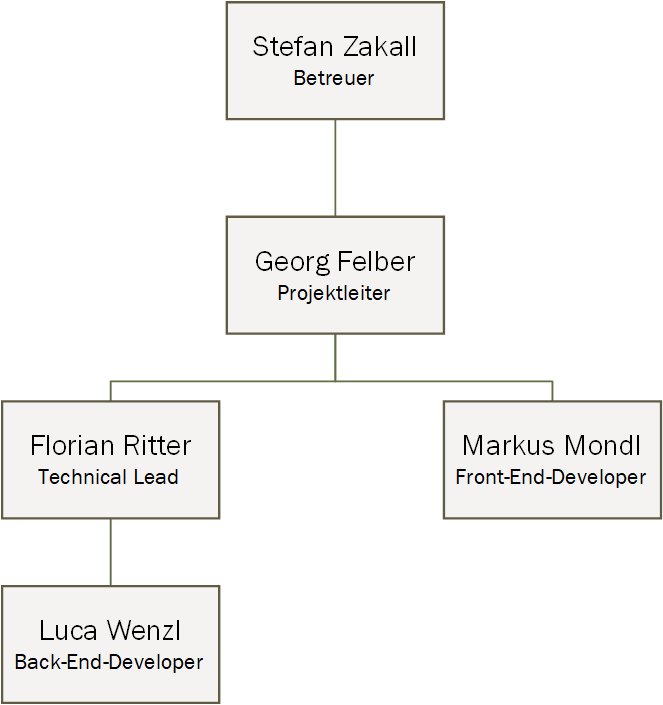
\includegraphics[width=.7\linewidth]{pictures/8.Projektorganisation/Projektteam.png}\
\caption{Projektteam}
\end{figure}
%\end{comment}
	% Markus
	\newpage
\section{Projektplanung}
Es wird der Projektstrukturplan mit den einzelnen Arbeitspaketen gezeigt. Ebenfalls wird der Balkenplan, welcher die Zeit für die jeweiligen Arbeitspakete benötigt wird, vorgestellt.
\subsection{Projektstrukturplan}
Die beiden Back-End-Developer sind für die Desktop-Version des Produkts als auch für die Applikation zuständig. Da sie   im Bereich des kabellosen Datentransfers nur wenig Erfahrung haben müssen sie sich während dem Projekt das Nötige Knowhow erarbeiten. Der Front-End-Developer kümmert sich um die GUI für die Desktop-Version und Applikation. Neben der Erstellung der Interfaces hat dieser auch die Aufgabe das Webportal für das Produkt zu erstellen. Um das beste Ergebnis zu erreichen wird das Projektteam interne Tests als auch eine Zielgruppentestung mit Passanten durchführen.\\
%\begin{comment}
\begin{figure}[H]
	\centering
	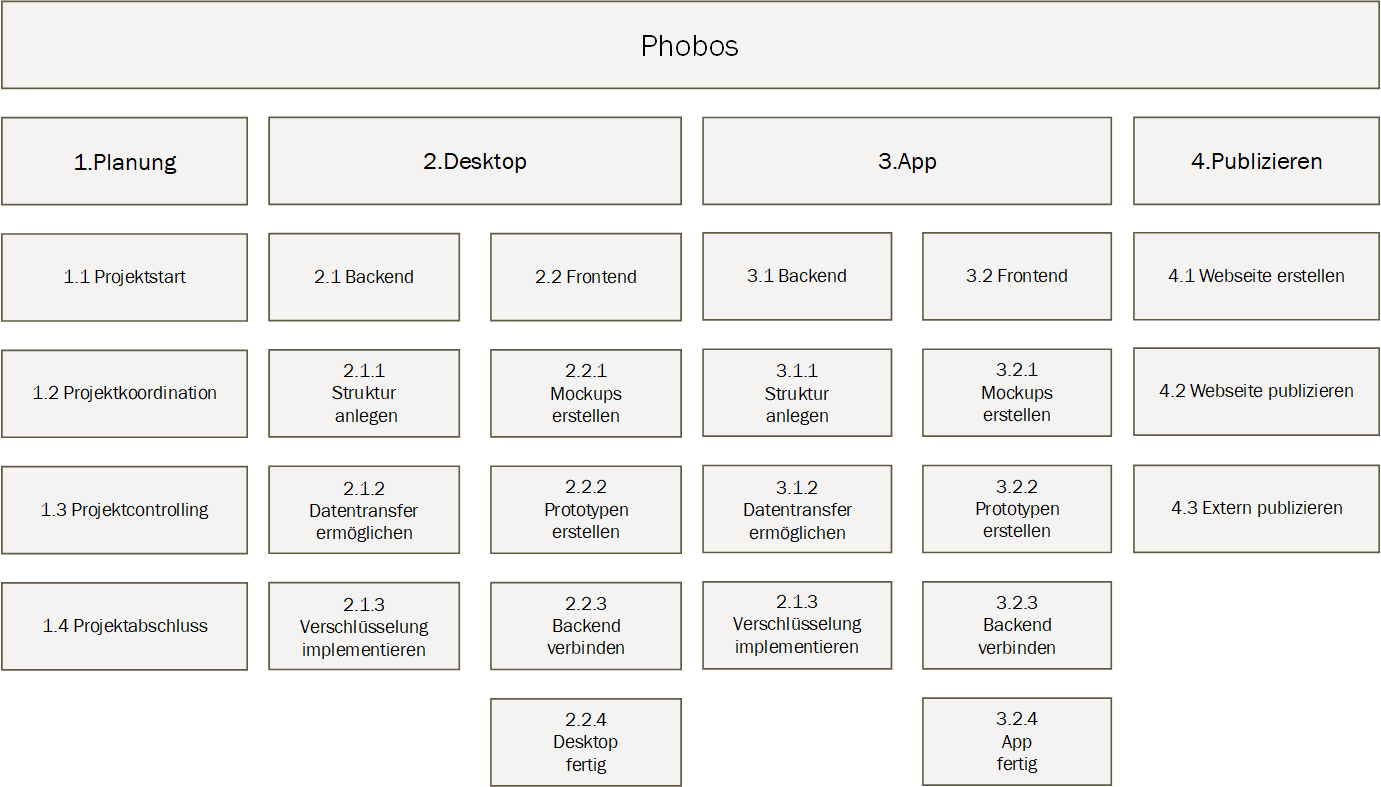
\includegraphics[width=\linewidth]{pictures/8.Projektorganisation/psp.png}\
	\caption{Projektstrukturplan}
\end{figure}
%\end{comment}
\newpage
\subsection{Balkenplan}
Die Arbeitspakete sollen zwischen dem 14.2.2019 und dem 23.05 abgeschlossen werden. Dabei werden 40 Prozent, also ca. 1 Monat, der Zeit für die Projektanfang, Lastenheft, Machbarkeitsstudie und Pflichtenheft, vorgesehen. Der Abschluss von Desktop und App Version werden in dessen Aufwand geplant 55 Prozent der Zeit in Anspruch nehmen. Die Publizierung des Produktes soll die letzten 5 Prozent benötigen.\\
%\begin{comment}
\begin{figure}[H]
\centering
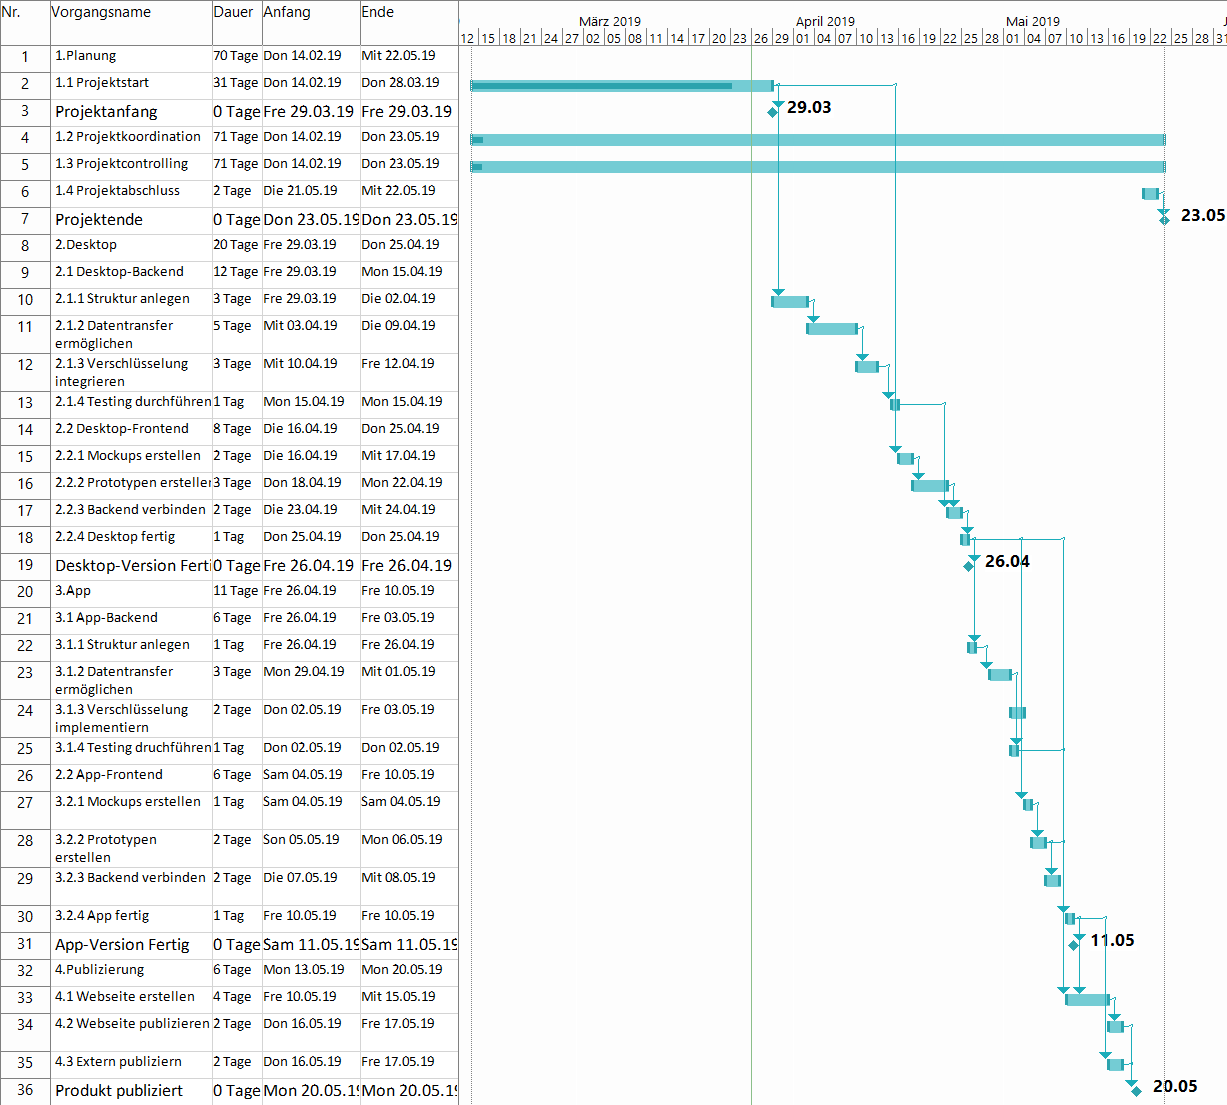
\includegraphics[width=\linewidth]{pictures/8.Projektorganisation/balkenplan.png}\
\caption{Balkenplan}
\end{figure}
%\end{comment}
\newpage
\subsection{Meilensteinplan}
Das Projekt soll voraussichtlich am 23.05.2019 beendet werden. Bis zu diesem Zeitpunkt hat das Projektteam 4 Meilensteine absolviert. Die Beschreibung, was genau bei diesen Meilensteinen abgeschlossen bzw. abgegeben wird, steht in der folgenden Tabelle.
\begin{table}[H]
	\begin{center}
		\begin{tabularx}{\linewidth}{|X|X|X|}
			\hline
			\textbf{Meilenstein}&Deliverable&Datum\\
			\hline
			Projektstart&Alle Dokumente mit den Informationen zum Projekt&Voraussichtlich 29.03.2019\\
			\hline
			Desktop-Version&Funktionsfähige Desktop-Applikation mit allen genannten Funktionen&Voraussichtlich 26.04.2019\\
			\hline
			Smartphone-Version&Funktionsfähige Smartphone-Applikation mit allen genannten Funktionen&Voraussichtlich 11.05.2019\\
			\hline
			Produkt publizieren&Funktionsfähige Webseite mit allen genannten Funktionen. Veröffentlichtes Produkt auf Google Play Store&Voraussichtlich 20.05.2019\\
			\hline
			Projektende&Fertiges Produkt wie vereinbart&Voraussichtlich 23.05.2019\\
			\hline
		\end{tabularx}
	\end{center}
\end{table}		% Markus
	\newpage
\section{Management Summary}
Wenn es während der Durchführung des Projekts zu keinen Problemen kommt wird es startend am 29.03.2019, in 70 Tagen am 23.05.2019 abgeschlossen und bereit zur Übergabe sein. Genauere Termine sind im Balkenplan als auch im Meilensteinplan zu sehen.
\\\\
Da keines der derzeit bekannten Übertragungssoftware den Kriterien entspricht, wird eine neue Software entwickelt. Ein Sinnvoller Ansatz bei der Umsetzung des Projekts ist die Auswahl einer populären Laufumgebung. Zu den meistbenutzten Laufumgebung im Smartphone-Bereich zählt Android und iOS. Im Bereich der Heimcomputer bzw. Laptops zählen Windows als auch Linux zu einen der meist benutzten Umgebungen. Es wurde entschieden das für das Projekt die Plattformen Windows, Linux als auch Android verwendet werden.
\\\\
Für die Umsetzung der Smartphone und Desktop Applikation wird die Programmiersprache Java verwendet. Das Know-How des Projektteams im Feld Java ist sehr gut und wird für das Projekt mehr als ausreichend sein. Durch diese bekannte Umgebung ist das Projekt für das Entwicklerteam technisch als auch persönlich machbar.
Bei der Verwirklichung des Projekts werden finanzielle Kosten auftreten welche bereits im Projektantrag erwähnt wurden und insgesamt einen Betrag von 200€ ausmachen.
\\\\
Abschließend kann man sagen, dass das Projekt durchführbar ist.				% Markus, Georg, Florian
	\section{Glossar}
Das \textbf{Backend} beschreibt die Schnittstelle zwischen einem Rechengerät und einer Software. Sie enthält die Funktionen, meist in einer Programmiersprache umgesetzt. Backend und Frontend sind zu unterscheiden.
\\
\\
\textbf{Windows 10} ist das aktuellste Betriebssystem der Microsoft Windows NT Serie. Es stellt ein System für ein Rechengerät dar.
\\
\\
\textbf{Android 8.0} oder auch 'Oreo' genannt. Ist die am häufigst genutzte Google Android Version, welche noch aktuell ist. Sie bietet ein Betriebssystem für Smartphones, jedoch nicht für Apple iPhones. Android ist meist OEM und kostenfrei.
\\
\\
\textbf{Debian 9} ist eine sehr beliebte Linux-Distribution, die noch oft im Einsatz von kleineren Firmen und Privatanwendern ist. Es ist ein kostenfreies Betriebssystem.
\\
\\
\textbf{macOS} ist das einzige Betriebssystem für Rechensysteme von Apple und wird nur für die Eigenmarken verwendet.
\\
\\
\textbf{iOS} ist das einzige Betriebssystem für Smartphones von Apple und wird ebenso nur für die Eigenmarken verwendet.
\\
\\
Mit dem \textbf{Frontend} wird die Schnittstelle zwischen der Software und dem Anwender beschrieben. Sie wird auch oft als grafische Darstellung einer Software bezeichnet.
\\
\\
Mit dem \textbf{Desktopinterface} ist das Frontend der Desktopapplikation gemeint.
\\
\\
Mit dem \textbf{Appinterface} ist das Frontend der App gemeint.
\\
\\
Der \textbf{Play Store} ist das Application-Prividing-System von Google auf dem Android-Betriebssystem.
\\
\\
Der \textbf{App Store} ist das Application-Providing-System von Apple auf dem macOS- und iOS-Betriebssystem.
\\
\\
\textbf{BlueTooth} beschreibt die Übertragungsschnittstelle, welche nur auf einem kleinen Bereich wirksam ist. Sie entspricht dem Standard IEEE 802.15.1.				% Florian
\end{document}